% Classe do documento e parâmetros gerais.
\documentclass[a4paper,openright,twoside,11pt]{report}

% Packages utilizadas e respetivos parâmetros.
\usepackage[utf8]{inputenc}
\usepackage[english]{babel}

\addto{\captionsenglish}{\renewcommand{\bibname}{References}}
\addto{\captionsenglish}{\renewcommand{\contentsname}{Contents}}
\addto{\captionsenglish}{\renewcommand{\appendixname}{Appendix}}

\usepackage{graphicx}
\usepackage{url}
\usepackage{float}
\usepackage{listings}
\usepackage{xcolor}
\usepackage{hyperref}
\usepackage{tabularx}
\usepackage{booktabs}
\usepackage{float}

\usepackage[Algoritmo]{algorithm}
\usepackage{algorithmicx}
\usepackage{algpseudocode}

\renewcommand{\algorithmicrequire}{\textbf{Dados: }}
\renewcommand{\algorithmicensure}{\textbf{Resultado: }}

% Definições das dimensões das páginas
\setlength{\textheight}{24.00cm}
\setlength{\textwidth}{15.50cm}
\setlength{\topmargin}{0.35cm}
\setlength{\headheight}{0cm}
\setlength{\headsep}{0cm}
\setlength{\oddsidemargin}{0.25cm}
\setlength{\evensidemargin}{0.25cm}

% Página inicial (capa)
\title{
   \vspace{-50mm}
   \begin{minipage}[l]{\textwidth}
      \hspace{-20mm}\resizebox{75mm}{!}{
\includegraphics{./figures/logoISELnew2.png}}\\
   \end{minipage}\\[20mm]

   {\bf DiárioLX — Plataforma Digital de Jornalismo Académico}
}

\author{
\begin{tabular}{ll}
             & Jessé Alencar  \\
             & Julianne Lobato \\[50mm]
\end{tabular}}

\date{
\begin{tabular}{ll}
  {Orientadores:} & Artur Ferreira \\
                  & Filipe Freitas\\
                  & Fátima Cardoso (ESCS)\\
\end{tabular}\\[10mm]
Relatório do projeto realizado no âmbito de Projecto e Seminário\\
Licenciatura em Engenharia Informática e de Computadores\\[20mm]
Junho de 2026}

\begin{document}
\pagenumbering{roman}
\thispagestyle{empty}
\maketitle

\baselineskip 18pt

% Contracapa
\newpage
\thispagestyle{empty}

% Página de assinaturas
\cleardoublepage
\setcounter{page}{1}

\begin{center}

  \textsc{\LARGE Instituto Superior de Engenharia de Lisboa}\\[50mm]

  {\large \bf DiárioLX — Plataforma Digital de Jornalismo Académico}\\[20mm]

  \begin{tabular}{rl}
    51745 & Jessé Alencar      \\[10mm]
          & \rule{75mm}{0.5pt} \\[5mm]

    51191 & Julianne Lobato    \\[10mm]
          & \rule{75mm}{0.5pt} \\
  \end{tabular}\\[10mm]

  \begin{tabular}{rl}
    Orientadores: & Artur Ferreira        \\[10mm]
                  & \rule{75mm}{0.5pt}    \\[5mm]

                  & Filipe Freitas        \\[10mm]
                  & \rule{75mm}{0.5pt}    \\[5mm]

                  & Fátima Cardoso (ESCS) \\[10mm]
                  & \rule{75mm}{0.5pt}    \\
  \end{tabular}\\[10mm]

  Relatório do projeto realizado no âmbito de Projecto e Seminário\\
  Licenciatura em Engenharia Informática e de Computadores\\[20mm]

  Junho de 2026\\

\end{center}

% Resumo
\cleardoublepage
\chapter*{Resumo}

O Diário LX é uma plataforma de jornalismo digital desenvolvida em colaboração com
a Escola Superior de Comunicação Social (ESCS) e a unidade de investigação LIACOM,
com o objetivo de suportar a criação, gestão e publicação de conteúdo editorial.
Foram avaliadas soluções existentes de gestão de conteúdos, nomeadamente o WordPress
e o Ghost; contudo, as suas arquitecturas e fluxos editoriais não satisfaziam
integralmente os requisitos do projeto, em particular o controlo de acessos baseado
em papéis, um fluxo de publicação estruturado, a integração de conteúdos multimédia
e uma arquitectura de aplicação desacoplada.

A solução proposta segue uma arquitectura cliente-servidor composta por um frontend
em React e um backend em Spring Boot implementado em Kotlin. O PostgreSQL foi adoptado
para a persistência de dados estruturados, enquanto os assets multimédia são
armazenados num serviço compatível com S3 auto-hospedado (SeaweedFS). A comunicação
entre componentes é realizada através de uma API REST, com respostas de erro a seguir
o standard Problem Details for HTTP APIs (RFC 9457).

A plataforma suporta um fluxo editorial no qual o conteúdo progride por estados
definidos --- rascunho, pendente de aprovação, publicado e rejeitado --- aplicado
por um modelo de permissões baseado em três níveis de utilizador: Colaborador,
Editor e Administrador. A autenticação é implementada através de JSON
Web Tokens (JWT), com tokens de acesso de curta duração e tokens de actualização de
longa duração armazenados em cookies \texttt{HttpOnly}, garantindo validação stateless
e mitigação de ataques XSS.

Este relatório descreve a versão beta do sistema, cobrindo as decisões de
arquitectura, modelo de dados, implementação do backend e frontend, e os testes
realizados até à data. A plataforma desenvolvida demonstra a viabilidade de uma
solução dedicada, adaptada aos fluxos editoriais e requisitos técnicos do Diário LX.

\vspace{5mm}
\textbf{Palavras-chave:} Jornalismo Digital; Sistemas de Gestão de Conteúdos;
Desenvolvimento Web; API REST; React; Spring Boot; Fluxo Editorial.

\cleardoublepage
\chapter*{Abstract}

Diário LX is a digital journalism platform developed in collaboration with the
Escola Superior de Comunicação Social (ESCS) and the LIACOM research unit, aimed
at supporting the creation, management, and publication of editorial content.
Existing content management systems such as WordPress and Ghost were evaluated as
potential solutions; however, their architectures and editorial workflows did not
fully address the project requirements, namely fine-grained role-based access
control, a structured publication workflow, multimedia integration, and a decoupled
application architecture.

The proposed solution follows a client-server architecture composed of a React-based
frontend and a Spring Boot backend implemented in Kotlin. PostgreSQL was adopted for
structured data persistence, while multimedia assets are stored through a self-hosted
S3-compatible service (SeaweedFS). Communication between components is performed
through a RESTful API, with error responses following the Problem Details for HTTP
APIs standard (RFC 9457).

The platform supports an editorial workflow in which content progresses through
defined states --- draft, pending approval, published, and rejected --- enforced by
a role-based permission model with three user levels: Contributor, Editor,
and Administrator. Authentication is implemented using JSON Web Tokens (JWT),
with short-lived access tokens and long-lived refresh tokens stored as \texttt{HttpOnly}
cookies, ensuring stateless validation and mitigation of XSS attacks.

This report describes the beta version of the system, covering the architectural
decisions, data model, backend and frontend implementation, and the testing carried
out to date. The resulting platform demonstrates the feasibility of a purpose-built
solution tailored to the editorial workflows and technical requirements of Diário LX.

\vspace{5mm}
\textbf{Keywords:} Digital Journalism; Content Management Systems; Web Development;
REST API; React; Spring Boot; Editorial Workflow.

% IA
\cleardoublepage
\chapter*{Usage of Generative AI Tools}

Throughout this project, generative artificial intelligence tools were used to support different stages of the development process. These tools were primarily employed for brainstorming technical solutions, exploring architectural approaches, assisting with documentation writing and structuring, and supporting the initial prototyping of certain interface components.

AI tools were also used to generate preliminary code examples, assist in the creation of Bootstrap-based layouts, and clarify technical concepts related to the technologies adopted in the project.

All final architectural, implementation, and validation decisions were made by the project authors.

% Índice
\cleardoublepage
\tableofcontents
\cleardoublepage

% Figuras e tabelas
\listoffigures
\cleardoublepage

\listoftables
\cleardoublepage

% Numeração normal
\setcounter{page}{1}
\pagenumbering{arabic}

% =========================
% CAPÍTULOS
% =========================

% Capítulo 1 — Introdução
%
% Chapter 1 — Introduction
%
\chapter{Introduction} \label{cap:intro}

\section{Context} \label{sec:intro_context}

In a media ecosystem increasingly marked by misinformation and the erosion of journalistic standards, \textit{Diário LX} emerges as a digital journalism initiative committed to editorial ethics, slow journalism, and proximity to local communities. The project is developed within the Journalism Trends Laboratory (\textit{Laboratório de Tendência no Jornalismo}), a structure affiliated with LIACOM (Applied Research Laboratory in Communication and Media) at the Escola Superior de Comunicação Social (ESCS) of the Instituto Politécnico de Lisboa (IPL).

The platform targets a young audience aged 18 to 35 years, with higher education backgrounds, and places a particular emphasis on the Greater Lisbon region. Editorially, it promotes visual journalism, long-form reporting, and investigative content, while deliberately avoiding clickbait-driven content strategies. The project has no commercial purpose and carries no advertising, operating instead with civic, educational, and scientific goals, co-funded by FCT (Fundação para a Ciência e Tecnologia).

\section{Motivation} \label{sec:intro_motivation}

A proof of concept was initially implemented using WordPress to validate the editorial structure and workflow. However, this approach revealed significant limitations in terms of architectural control, customization, and long-term scalability. The need to build a purpose-built platform that fully supports the editorial lifecycle — from content creation and review to publication and archival — motivated the development of this system from the ground up.

\section{Solution Overview} \label{sec:intro_solution}

\textit{Diário LX} is a web-based content management and publication platform
built to support the full editorial lifecycle of a digital journalism
outlet. The system is organized around two distinct areas:

\begin{itemize}
      \item \textbf{Backoffice}: A restricted editorial management interface, accessible only to authenticated users (Administrators, Editors, and Contributors), supporting content creation, revision, approval, and publishing workflows.
      \item \textbf{Public Website}: A reader-facing interface providing access to published articles, multimedia content (podcasts, videos, photo essays), organized by category, tag, and editorial section.
\end{itemize}

The system is built around an editorial workflow in which content progresses through
defined states — draft, pending review, published, and rejected — with each transition
guarded by the requesting user's role.

\section{Report Organization} \label{sec:intro_organization}

The remainder of this report is organized as follows:

\begin{itemize}
      \item Chapter~\ref{cap:background} presents the context, related work, and existing solutions analysed during the project.
      \item Chapter~\ref{cap:requirements} details the functional and non-functional requirements of the system.
      \item Chapter~\ref{cap:architecture} describes the system architecture and technology choices.
      \item Chapter~\ref{cap:datamodel} presents the data model.
      \item Chapter~\ref{cap:backend} covers the backend implementation.
      \item Chapter~\ref{cap:frontend} covers the frontend implementation.
      \item Chapter~\ref{cap:deployment} describes how the system is packaged and deployed to production.
      \item Chapter~\ref{cap:conclusion} concludes the report, summarising the delivered system and outlining directions for future work.
\end{itemize}


% Capítulo 2 — Problema e Contexto
%
% Chapter 2 — Background and Related Work
%
\chapter{Background} \label{cap:background}

\section{Digital Journalism Platforms} \label{sec:background_journalism}

Digital journalism has undergone significant transformations in the past decade, driven
by the proliferation of social media, mobile devices, and algorithmic content
distribution. Traditional newsrooms have increasingly migrated to web-native platforms,
yet many existing solutions prioritise speed and volume over editorial rigour and
journalistic depth~\cite{slow_journalism}.

Slow journalism, as a counter-movement, emphasises long-form reporting, investigative
depth, and contextual analysis. Platforms designed to support slow journalism require
features that differ substantially from high-volume news aggregators: robust editorial
workflows, multimedia support, and fine-grained access control for editorial teams.

\section{Existing Solutions} \label{sec:background_existing}

Several content management systems (CMS) were analysed as potential off-the-shelf
solutions before the decision was made to develop a bespoke platform.

\subsection{WordPress} \label{sec:background_wordpress}

WordPress is the most widely adopted CMS in the world, powering over 40\% of all
websites~\cite{wordpress_stats}. A WordPress-based proof of concept was the starting
point for this project. Although WordPress provides a rich plugin ecosystem and a
familiar editorial interface, it presents notable limitations in the context of
Diário LX:

\begin{itemize}
      \item Limited control over the editorial approval workflow without heavy plugin
            dependencies.
      \item Performance and security concerns at scale.
      \item Architectural rigidity that complicates custom API design and frontend
            decoupling.
\end{itemize}

\subsection{Ghost} \label{sec:background_ghost}

Ghost~\cite{ghost_cms} is a modern, open-source publishing platform focused on independent journalism
and newsletters. It offers a clean editorial interface and native support for
membership models. Ghost defines four built-in roles --- \textit{Contributor},
\textit{Author}, \textit{Editor}, and \textit{Administrator} --- with well-defined
publish permissions. Contributors cannot publish directly and must submit content for
review. However, Ghost does not support explicit content rejection: editors can only
publish or leave content unpublished, with no formal rejection state or feedback
mechanism for contributors. This makes it unsuitable for a newsroom where editorial
accountability and structured feedback are part of the workflow. Its theming system
also makes full frontend decoupling impractical.

\subsection{Summary} \label{sec:background_summary}

The three platforms differ significantly in how they address the core requirements
of Diário LX.

Regarding \textbf{editorial workflow}, WordPress requires plugins to approximate any
structured content lifecycle, while Ghost supports a basic submit-and-publish model
where Contributors cannot publish directly but editors have no formal way to reject
content --- they can only publish or leave it unpublished, with no feedback mechanism
for contributors. Diário LX enforces a formal lifecycle with four explicit states ---
\textit{Draft}, \textit{Pending}, \textit{Published}, and \textit{Rejected} ---
requiring an editor to explicitly approve or reject each submission before publication.

Regarding \textbf{role-based access control}, WordPress relies on plugins for any
granular permission model. Ghost defines four built-in roles with well-defined publish
restrictions, but the permissions are tied to the platform's own publishing model and
cannot be extended. Diário LX defines three roles --- \textit{Contributor},
\textit{Editor}, and \textit{Administrator} --- enforced directly at the API level,
meaning every endpoint independently validates the caller's role without depending on
any plugin or external system.

Regarding \textbf{multimedia support}, both WordPress and Ghost treat multimedia as
a secondary concern, relying on basic media libraries or plugins. Diário LX includes
a native upload pipeline supporting images, video, and audio, with direct integration
into the content authoring workflow.

Regarding \textbf{frontend decoupling}, WordPress and Ghost both tie the presentation
layer to their own theming systems, which constrains the design and technology choices
available to the frontend. Diário LX exposes a dedicated REST API consumed by an
independent React application, meaning the frontend can be developed, deployed, and
replaced entirely without touching the backend.

Table~\ref{tab:cms_comparison} consolidates these differences.

\begin{table}[H]
      \centering
      \caption{Comparison of existing CMS solutions against Diário LX requirements.}
      \label{tab:cms_comparison}
      \begin{tabularx}{\textwidth}{lXXX}
            \toprule
            \textbf{Feature}   & \textbf{WordPress} & \textbf{Ghost}        & \textbf{Diário LX}      \\
            \midrule
            Editorial workflow & Plugin-based       & Submit/publish only,  & Draft → Pending →       \\
                               &                    & no rejection state    & Published / Rejected    \\
            \addlinespace
            Role-based access  & Plugin-based       & Four built-in roles,  & Three roles, enforced   \\
                               &                    & no rejection feedback & natively at API level   \\
            \addlinespace
            Multimedia support & Plugin-based       & Basic                 & Native (images, video,  \\
                               &                    &                       & audio)                  \\
            \addlinespace
            API-first design   & Partial            & Yes                   & Yes                     \\
            \addlinespace
            Custom frontend    & Theme-based        & Theme-based           & React (fully decoupled) \\
            \addlinespace
            Open source        & Yes                & Yes                   & Yes                     \\
            \bottomrule
      \end{tabularx}
\end{table}

None of the analysed off-the-shelf solutions fully satisfies the editorial workflow,
access control, and multimedia management requirements of Diário LX, motivating the
development of a purpose-built platform.

% Capítulo 3 — Requisitos do Sistema
%
% Chapter 3 — System Requirements
%
\chapter{System Requirements} \label{cap:requirements}

This chapter presents the functional and non-functional requirements of the Diário LX platform, derived from the project specification and validated with the editorial team.

\section{Functional Requirements} \label{sec:req_functional}

\subsection{Content Management} \label{sec:req_content}

The system must provide a full content management lifecycle supporting the following content types: \textbf{articles}, \textbf{podcasts}, \textbf{videos}, and \textbf{photo essays}. Each content item must include the following attributes:

\begin{itemize}
  \item Title
  \item Body text (supporting inline subtitles, highlights, and captioned images)
  \item Lead paragraph (\textit{entrada})
  \item Author(s) and photo author
  \item Creation and publication date
  \item Featured image
  \item Category and subcategory
  \item Tags
\end{itemize}

Content must progress through a defined workflow:

\begin{enumerate}
  \item \textbf{Draft} — created and edited by a Contributor.
  \item \textbf{Pending Approval} — submitted for editorial review.
  \item \textbf{Published} — approved and publicly visible.
  \item \textbf{Rejected} — returned to the author with revision comments.
\end{enumerate}

It must be possible to archive and permanently delete content. Media file uploads are limited to 2\,GB. It must be possible to mark content as featured for display on the homepage.

\subsection{Categories, Subcategories, and Tags} \label{sec:req_categories}

Content must be organised using categories and subcategories. The main editorial sections are:

\begin{itemize}
  \item Lisboa, Cidade Aberta
  \item A Fundo
  \item Secções (Mundo, Política, Sociedade, Economia, Cultura e Media, Bem-Viver, Desporto)
  \item Especiais
  \item Fotografia
  \item Podcasts
  \item Vídeos
\end{itemize}

Each category must support a name, an associated colour, and an automatically generated listing page. Tags must also have dedicated listing pages. The system must allow the creation, editing, and deletion of categories and tags.

\subsection{User Management and Permissions} \label{sec:req_users}

The system defines three user roles:

\begin{description}
  \item[Administrator] Full system control: manages users, system settings, approves or rejects content and new accounts, and has access to all backoffice areas.
  \item[Editor] Can approve or reject submitted content, manage contributor accounts, and deactivate users.
  \item[Contributor] Can create and submit content for approval. Cannot publish directly.
\end{description}

Each user profile includes: name, email, profile photograph, active/inactive status, professional function (journalist or photographer), and role.

\subsection{Backoffice} \label{sec:req_backoffice}

The backoffice must provide:

\begin{itemize}
  \item Account creation for Editors and Contributors.
  \item Login and logout for all profiles.
  \item Listing and search of all articles and users.
  \item Profile editing (own profile for all; any profile for Administrators).
  \item Comment moderation (approve, reject, hide) by Administrators and Editors.
\end{itemize}

\subsection{Public Website} \label{sec:req_frontend}

\subsubsection{Homepage}
The homepage must display:
\begin{itemize}
  \item 4 featured articles (defined in the backoffice).
  \item The 4 most recent articles.
  \item Navigation to main editorial sections.
  \item Links to institutional pages: Team, Editorial Statute, and Code of Ethics.
\end{itemize}

\subsubsection{Other Pages}
\begin{itemize}
  \item \textbf{Category page}: one featured article (defined in the backoffice) and remaining articles in reverse chronological order.
  \item \textbf{Tag page}: list of associated articles.
  \item \textbf{Article page}: full article view, reader comments, and 4 related articles.
  \item \textbf{Team page}.
  \item \textbf{Podcast page}: dedicated layout distinct from other category pages.
\end{itemize}

\subsection{Search and Navigation} \label{sec:req_search}

\begin{itemize}
  \item Full-text keyword search across articles.
  \item Human-readable, slugified URLs (e.g. \texttt{/politica/orcamento-estado-2026}).
\end{itemize}

\subsection{Compatibility} \label{sec:req_compat}

The system must be compatible with modern browsers and fully functional on mobile devices (responsive design for mobile, tablet, and desktop viewports).

\section{Non-Functional Requirements} \label{sec:req_nonfunctional}

\begin{itemize}
  \item \textbf{Security}: Authentication via token-based mechanism; role-based access control enforced at the API level.
  \item \textbf{Performance}: Pages must load within acceptable response times under expected editorial team and reader load.
  \item \textbf{Maintainability}: Codebase organised to allow independent evolution of frontend and backend.
  \item \textbf{Media storage}: Support for images, audio (podcasts), and video files up to 2\,GB per upload.
  \item \textbf{Scalability}: Architecture must support growth in both content volume and concurrent users.
\end{itemize}

\section{Optional Requirements} \label{sec:req_optional}

The following features are considered optional and may be addressed in future iterations:

\begin{itemize}
  \item Scheduled publication of content.
  \item Advanced search filters (by date, category, author, tag) in both backoffice and public site.
  \item User search filters in the backoffice (by role, function, status).
  \item Reader account registration and commenting.
  \item Audiodescription support for visually impaired users.
  \item Multilingual support (Portuguese and English).
\end{itemize}


% Capítulo 4 — Arquitetura
%
% Chapter 4 — Architecture
%
\chapter{Architecture} \label{cap:architecture}

\section{Overview} \label{sec:arch_overview}

The Diário LX platform follows a client-server architecture. The system is composed of a browser-executed client application and a server-side infrastructure responsible for business logic and data management. Figure~\ref{fig:architecture} illustrates the high-level architecture of the system.

% TODO: inserir figura da arquitetura
\begin{figure}[H]
  \begin{center}
    % \resizebox{130mm}{!}{\includegraphics{./figures/architecture.png}}
    \framebox[130mm]{\rule{0pt}{60mm} Architecture Diagram (Figure placeholder)}
  \end{center}
  \caption{High-level system architecture.}
  \label{fig:architecture}
\end{figure}

The system comprises the following main components:

\begin{itemize}
  \item \textbf{React Client}: A single-page application (SPA) running in the browser, responsible for rendering the public website and the backoffice interface.
  \item \textbf{Reverse Proxy}: Serves static assets and routes HTTP requests to the appropriate backend service.
  \item \textbf{Spring Boot API}: The backend application, developed in Kotlin, responsible for all business logic, authentication, and data access.
  \item \textbf{PostgreSQL Database}: Relational database storing structured data (articles, users, categories, tags).
  \item \textbf{Media Storage}: Dedicated storage system for multimedia files (images, audio, video). The specific provider is to be decided.
\end{itemize}

\section{Technology Stack} \label{sec:arch_stack}

Table~\ref{tab:tech_stack} summarises the technologies adopted in this project.

\begin{table}[H]
  \centering
  \caption{Technology stack.}
  \label{tab:tech_stack}
  \begin{tabularx}{\textwidth}{llX}
    \toprule
    \textbf{Layer} & \textbf{Technology}  & \textbf{Rationale}                                                      \\
    \midrule
    Frontend       & React (TypeScript)   & Component-based UI architecture and strong ecosystem support            \\

    Backend        & Spring Boot (Kotlin) & Robust HTTP API development, JVM ecosystem integration, and type safety \\

    Database       & PostgreSQL           & Relational model well-suited for editorial and multimedia data          \\

    Reverse Proxy  & Nginx                & Standard and performant reverse proxy and static asset serving          \\

    Media Storage  & SeaweedFS            & S3-compatible distributed storage with low operational overhead         \\

    Authentication & Bearer Tokens        & Server-side token invalidation and simplified session management        \\

    \bottomrule
  \end{tabularx}
\end{table}

\section{API Design} \label{sec:arch_api}

Communication between the frontend and backend is handled through a RESTful HTTP API. All endpoints are prefixed with \texttt{/api/v1/}. The API follows standard HTTP conventions for resource naming and status codes.

% TODO: listar ou referenciar os principais grupos de endpoints (artigos, utilizadores, categorias, etc.)

\section{Authentication and Authorization} \label{sec:arch_auth}

Authentication is implemented using a token-based mechanism (JWT). Upon successful login, the server issues a signed token that the client includes in subsequent requests via the \texttt{Authorization} header. Role-based access control (RBAC) is enforced at the API level: each endpoint validates the token and the caller's role before executing the requested operation.

\section{Editorial Workflow} \label{sec:arch_workflow}

Figure~\ref{fig:workflow} illustrates the publication lifecycle of a content item within the system.

% TODO: inserir figura do workflow
\begin{figure}[H]
  \begin{center}
    \framebox[130mm]{\rule{0pt}{50mm} Editorial Workflow Diagram (Figure placeholder)}
  \end{center}
  \caption{Publication workflow state machine.}
  \label{fig:workflow}
\end{figure}

Content transitions between the following states:

\begin{description}
  \item[Draft] Initial state. The content is only visible to its author.
  \item[Pending Approval] The author submits the content for review. It becomes visible to Editors.
  \item[Published] An Editor approves the content; it becomes publicly accessible.
  \item[Rejected] An Editor rejects the content, optionally providing revision comments. The author may edit and resubmit.
\end{description}

Editors and Administrators bypass the approval step and may publish content directly.


% Capítulo 5 — Modelo de Dados
%
% Chapter 5 — Data Model
%
\chapter{Data Model} \label{cap:datamodel}

\section{Entities} \label{sec:dm_entities}

This section describes the core entities of the Diário LX data model, their
attributes, and the relationships between them. The complete entity-relationship
diagram is presented in Appendix~\ref{app:db_model}.

\subsection{User} \label{sec:dm_user}

Represents an authenticated system user. Each user has a \texttt{user\_role}
(\textit{ADMIN}, \textit{EDITOR}, or \textit{CONTRIBUTOR}), credentials
(\texttt{username}, \texttt{email}, \texttt{password\_hash}), profile information
(\texttt{first\_name}, \texttt{last\_name}, \texttt{bio}), and an optional
\texttt{avatar\_media\_id} reference to a media item. An \texttt{active\_account}
flag is used to deactivate access without deleting the record.

\subsection{Session} \label{sec:dm_session}

Stores active refresh tokens issued upon login. Each session is associated with a
user and holds a \texttt{refresh\_token}, \texttt{created\_at}, and
\texttt{expires\_at}. Sessions are deleted on logout and expire automatically based
on \texttt{expires\_at}.

\subsection{Invite} \label{sec:dm_invite}

Represents an invitation token generated by an Administrator to allow new user
registration. Each invite carries a \texttt{role\_assigned}, an expiration
timestamp, and a \texttt{used} flag to prevent reuse.

\subsection{Content} \label{sec:dm_content}

The central entity of the system. Each content item has a \texttt{content\_type}
(\textit{ARTICLE}, \textit{VIDEO}, \textit{EPISODE}, or \textit{PODCAST}), a
\texttt{title}, a \texttt{headline}, a \texttt{slug}, and a reference to its
\texttt{category}. The body of a content item is composed of an ordered sequence
of \texttt{content\_blocks}.

The \texttt{published\_at} timestamp controls content visibility. When set to a
past value, the content is immediately publicly accessible. When set to a future
value, the content is scheduled for publication --- it has been approved but will
only become visible once that timestamp is reached. A \texttt{NULL} value indicates
the content has not yet been approved for publication.

Content items may have one or more authors, recorded in the \texttt{content\_authors}
association table with a \texttt{role} of \textit{primary} or \textit{secondary}.
A partial unique index ensures that each content item has at most one primary author.

\subsection{Content Block} \label{sec:dm_block}

Represents a single unit of content within a content item. Each block has a
\texttt{type} (\textit{text}, \textit{quote}, or \textit{image}), a
\texttt{position} defining its order within the content item, and either a
\texttt{content} text field (for text and quote blocks) or a \texttt{media\_id}
reference (for image blocks). A database constraint enforces that text and quote
blocks must have \texttt{content} set, and image blocks must have \texttt{media\_id}
set.

\subsection{Category} \label{sec:dm_category}

Editorial categories support a two-level hierarchy via a \texttt{parent\_id}
self-reference on the \texttt{categories} table. Top-level categories have
\texttt{parent\_id = NULL}; subcategories reference their parent. Each category
has a \texttt{name}, a unique \texttt{slug}, a unique \texttt{color}, and an
optional \texttt{description}. Categories may be soft-deleted via an
\texttt{archived\_at} timestamp.

\subsection{Tag} \label{sec:dm_tag}

Tags provide cross-cutting thematic classification. A content item may have multiple
tags, recorded in the \texttt{content\_tags} association table. Each tag association
carries a \texttt{role} of \textit{primary} or \textit{secondary}; a partial unique
index ensures that each content item has at most one primary tag.

\subsection{Media} \label{sec:dm_media}

Stores metadata for uploaded media files (images, videos, and audio). Binary files
are not stored in the database --- only their \texttt{bucket}, \texttt{object\_key},
\texttt{mime\_type}, \texttt{size\_bytes}, and a \texttt{status} field
(\textit{pending} or \textit{ready}) are persisted. The \textit{pending} state
indicates that the frontend has initiated the upload but not yet confirmed it; the
backend transitions the status to \textit{ready} upon confirmation.

Media items may have associated credits via the \texttt{media\_credits} table,
which records the contributing user and their \texttt{credit\_role}
(e.g.\ \textit{PHOTOGRAPHER}, \textit{VIDEOGRAPHER}, \textit{AUDIOGRAPHER}).

\subsection{Featured Content} \label{sec:dm_featured}

The \texttt{featured\_contents} table stores curated content selections for the
homepage. Each entry has a \texttt{key} identifying the slot (e.g.\
\texttt{homepage\_hero}, \texttt{lisboa\_featured}), a mandatory \texttt{content\_id}
reference to the selected content item, and a \texttt{position} for ordering within
the same slot group.

\section{Database Views} \label{sec:dm_views}

Several PostgreSQL views are defined to encapsulate complex query logic and provide
pre-joined representations of the data for use by the repository layer:

\begin{description}
      \item[\texttt{v\_contents}] Full content view, including category, featured media,
            authors ordered by role, tags, and content blocks with their associated media.
            Used for single content item retrieval.

      \item[\texttt{v\_contents\_summary}] Lightweight content listing view, including
            only the fields required for listing pages: title, slug, type, category,
            featured image URL, primary tag, and author names. Used for paginated content
            listings.

      \item[\texttt{v\_medias}] Media view that computes the full \texttt{url} and
            \texttt{thumbnail\_url} from \texttt{bucket} and \texttt{object\_key}, and
            aggregates credits as a JSON array.

      \item[\texttt{v\_categories}] Category view that joins each category with its
            parent name and includes a \texttt{quantity} count of associated content items.

      \item[\texttt{v\_tags}] Tag view that includes a \texttt{quantity} count of
            associated content items.
\end{description}

\section{Indexes} \label{sec:dm_indexes}

The following indexes were defined to support the most frequent query patterns:

\begin{description}
      \item[\texttt{idx\_content\_category\_id}] Supports filtering content by category.

      \item[\texttt{idx\_content\_blocks\_content\_position}] Composite index on
            \texttt{(content\_id, position)}, supporting ordered block retrieval per
            content item.

      \item[\texttt{idx\_content\_authors\_content\_id} and \texttt{idx\_content\_authors\_author\_id}]
            Support join queries on the \texttt{content\_authors} association table.

      \item[\texttt{uq\_content\_primary\_author}] Partial unique index ensuring that
            each content item has at most one author with \texttt{role = 'primary'}.

      \item[\texttt{uq\_content\_primary\_tag}] Partial unique index ensuring that
            each content item has at most one tag with \texttt{role = 'primary'}.
\end{description}

\section{Key Design Decisions} \label{sec:dm_decisions}

\begin{itemize}
      \item \textbf{Block-based content model}: Instead of storing article body as a
            single rich-text blob, content is decomposed into an ordered sequence of
            typed blocks (\textit{text}, \textit{quote}, \textit{image}). This enables
            structured rendering, easier reordering, and per-block media references.

      \item \textbf{Self-referencing category hierarchy}: A single \texttt{categories}
            table with a \texttt{parent\_id} foreign key supports the two-level category
            hierarchy without requiring a separate \texttt{subcategories} table.

      \item \textbf{Media metadata separation}: Binary files are stored in SeaweedFS;
            only metadata is persisted in the database. The \textit{pending}/\textit{ready}
            status tracks the asynchronous upload lifecycle, ensuring that incomplete
            uploads do not surface in the application before the file is available in
            storage.

      \item \textbf{Timestamps as epoch integers}: All timestamps are stored as
            \texttt{BIGINT} Unix epoch values rather than \texttt{TIMESTAMP} columns.
            This avoids timezone conversion issues, as epoch values are inherently UTC,
            and simplifies interoperability with the \texttt{kotlinx.datetime.Instant}
            type used throughout the backend.

      \item \textbf{Serial primary keys}: All tables use \texttt{SERIAL}
            (auto-incrementing integer) primary keys rather than UUIDs. This simplifies
            joins and keeps index sizes small, which is well-suited to the expected data
            volume of the platform.
\end{itemize}

% Capítulo 6 — Backend
\chapter{Backend} \label{cap:backend}

\section{Organization} \label{sec:be_organization}

The backend is a Spring Boot application written in Kotlin, structured as a set of
loosely coupled Gradle modules. Each module has a well-defined responsibility and
depends only on modules below it in the hierarchy, ensuring that business logic
remains isolated from infrastructure concerns, following principles commonly associated
with Clean Architecture~\cite{martin2017clean}. Figure~\ref{fig:backend_layers}
illustrates the module organization and the dependency relationships between them.

\begin{figure}[H]
      \begin{center}
            \resizebox{\textwidth}{!}{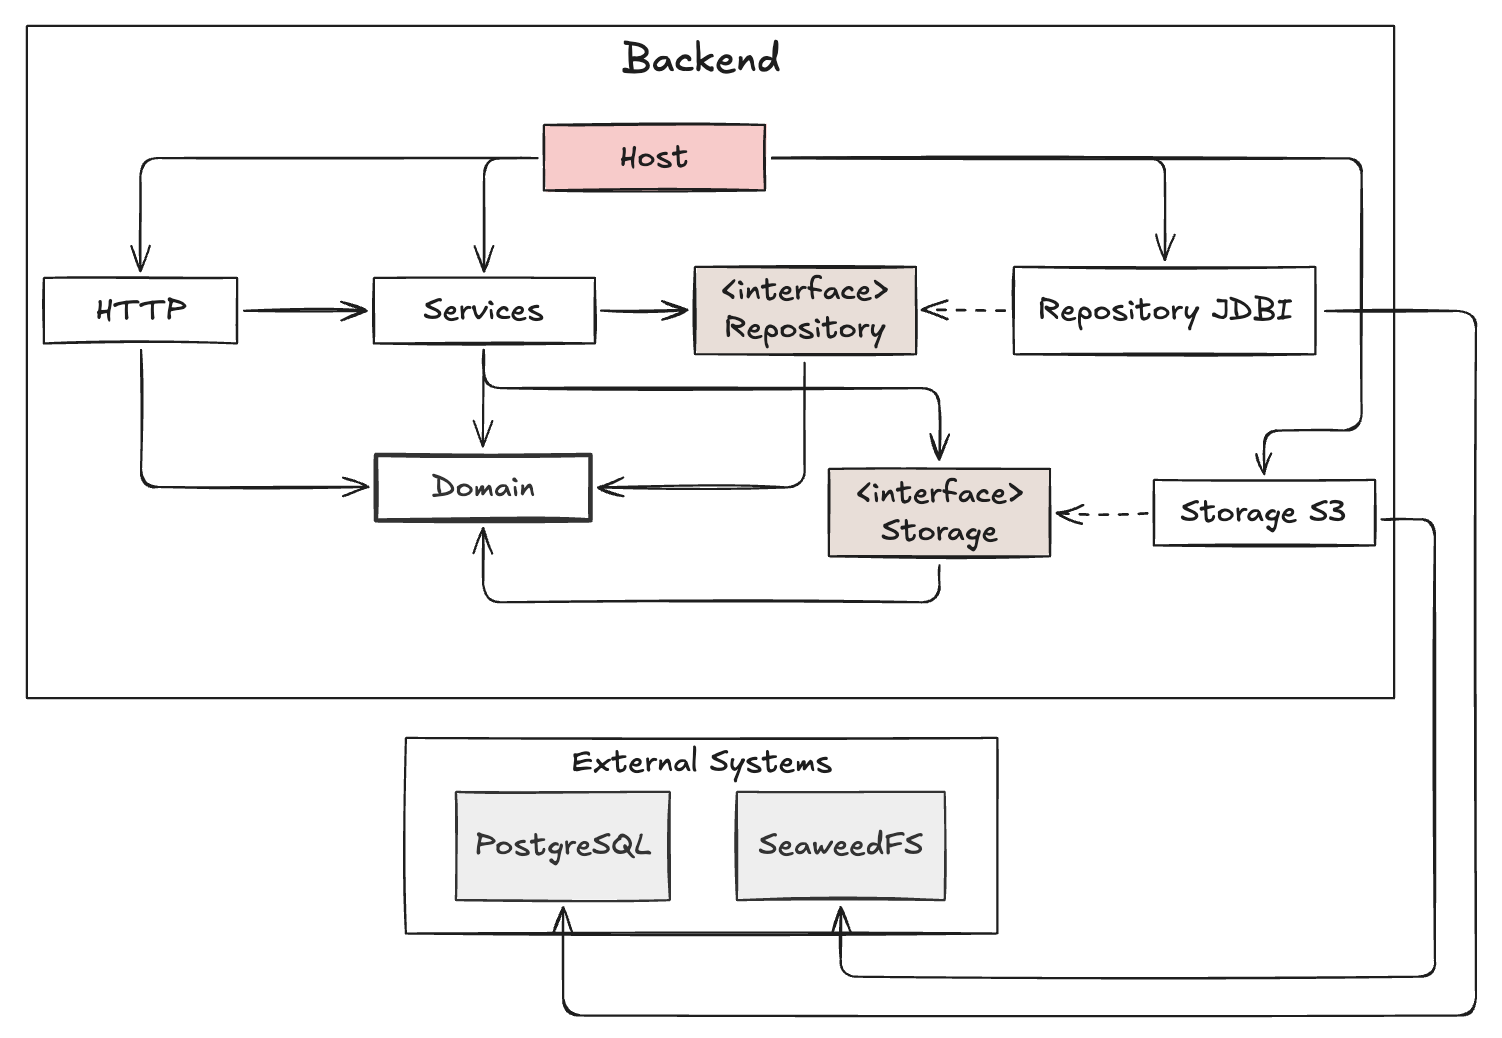
\includegraphics{./figures/backend_module_diagram.png}}
      \end{center}
      \caption{Backend module organization.}
      \label{fig:backend_layers}
\end{figure}

\begin{description}
      \item[HTTP] Defines the REST controllers that expose the API endpoints, each
            responsible for a bounded domain area (e.g., \texttt{ContentController},
            \texttt{UserController}, \texttt{CategoryController}). Also contains the
            authentication interceptor, argument resolvers, and Problem+JSON error handling.

      \item[Services] Contains the business logic, orchestrating operations across
            repositories and enforcing domain rules such as publication workflow transitions
            and permission checks.

      \item[Domain] Defines the core domain entities and value objects. This module
            has no dependencies on any other module, ensuring the domain model remains
            isolated from infrastructure concerns.

      \item[Repository] Defines the repository interfaces through which the service
            layer accesses persistent data. The concrete implementation, \texttt{Repository JDBI},
            implements these interfaces using JDBI, mapping SQL result sets to domain objects.
            This abstraction allows the persistence layer to be replaced without affecting
            business logic.

      \item[Storage] Defines the storage interface for multimedia files. The concrete
            implementation, \texttt{Storage S3}, integrates with SeaweedFS
            for binary file storage using the AWS S3 SDK~\cite{aws_s3_sdk}, as SeaweedFS
            exposes an S3-compatible API. An S3-compatible storage layer was chosen to
            avoid coupling the application to a specific storage provider while retaining a
            widely adopted interface. SeaweedFS was selected as a self-hosted
            implementation that satisfies the project's operational constraints and
            supports direct browser uploads, allowing large media files to bypass the
            application server during transfer. This approach reduces server load and keeps
            the backend responsible only for media metadata and access control.

      \item[Host] The root composition module, responsible for assembling the full
            application. It contains the Spring Boot entry point, all bean definitions, and
            the application configuration (database connection, storage credentials, server
            settings). No business logic resides here --- its sole purpose is wiring all
            modules together and bootstrapping the application.
\end{description}

The external systems used by the backend are \textbf{PostgreSQL}, accessed via the
JDBI repository implementation, and \textbf{SeaweedFS}, accessed via the S3 storage
implementation.

\section{Authentication} \label{sec:be_auth}

The authentication mechanism is described in Section~\ref{sec:arch_auth}. This
section covers the implementation details.

\subsection{JwtTokenGenerator} \label{sec:be_jwt}

Token generation and validation are handled by the \texttt{JwtTokenGenerator} class,
which encapsulates all JWT logic. Access tokens carry an HMAC-SHA256 message
authentication code (MAC), computed with a configurable secret key loaded at startup
via \texttt{JwtConfig}. The MAC key is initialised lazily and reused across requests. Refresh tokens are generated as
cryptographically random 32-byte strings encoded in Base64URL format using
\texttt{java.security.SecureRandom}.

\subsection{AuthenticationInterceptor} \label{sec:be_auth_interceptor}

The \texttt{AuthenticationInterceptor} implements Spring's \texttt{HandlerInterceptor}
interface, running before each request reaches a controller via the \texttt{preHandle}
method. It performs the following sequential checks:

\begin{enumerate}
      \item \textbf{Token extraction}: the interceptor reads the access token from the
            request cookies. If the endpoint requires authentication --- determined by the
            presence of a \texttt{@RequireRole} annotation or an \texttt{AuthenticatedUser}
            parameter --- and no valid token is found, the request is rejected with
            \texttt{401 Unauthorized}.

      \item \textbf{Role verification}: if the endpoint is annotated with
            \texttt{@RequireRole}, the role claim extracted from the JWT is compared against
            the required role without a database lookup. A mismatch results in a
            \texttt{403 Forbidden} response.
\end{enumerate}

If both checks pass, and the controller declares an \texttt{AuthenticatedUser}
parameter, the user is fetched from the database by the identifier in the JWT claims
and injected via \texttt{AuthenticatedUserArgumentResolver}. Endpoints that do not
declare this parameter incur no database lookup during authentication.

\section{Authorization} \label{sec:be_authorization}

Role-based access control (RBAC) is enforced at the HTTP layer via the
\texttt{@RequireRole} annotation. Each endpoint declares the minimum role required
to access it. The three roles --- \textit{Contributor}, \textit{Editor}, and
\textit{Administrator} --- form a strict permission hierarchy where each role inherits
all permissions of the roles below it, as described in
Section~\ref{sec:req_users}.

The adoption of a dedicated authorization library, such as Casbin~\cite{casbin}, was
considered as an alternative to enforcing the rules natively. General-purpose
authorization frameworks provide policy engines capable of expressing rich and
dynamic rule sets --- including attribute-based and relationship-based models --- and
are particularly valuable when access-control requirements are numerous, subject to
frequent change, or intended to be configurable at runtime without redeployment. In
the case of \textit{Diário LX}, however, the authorization model is deliberately small and
stable: it comprises three well-defined, hierarchically ordered roles whose
permissions are known at design time and are not expected to change. Under these
conditions, the expressive power of a policy engine offers limited practical benefit,
while introducing an additional external dependency, a separate policy definition to
maintain, and a layer of indirection between an endpoint and the rule that governs it.
Enforcing the rules natively through the \texttt{@RequireRole} annotation instead
keeps each endpoint's access requirement explicit and co-located with its declaration,
which favours readability and auditability. Adopting a library such as Casbin remains
a sensible evolution should the permission model grow in complexity --- for instance,
with per-resource ownership rules or finer-grained, runtime-configurable permissions
--- but for the current scope the additional complexity was not warranted.

\section{Error Handling} \label{sec:be_errors}

Error responses follow the \textbf{Problem Details for HTTP APIs} standard~\cite{rfc9457},
defined in RFC 9457. All error responses are returned with the
\texttt{application/problem+json} content type and contain the following fields:

\begin{itemize}
      \item \texttt{type} --- a URI identifying the problem type, pointing to the
            project's documentation at \texttt{github.com/jfmalencar/DiarioLX}.
      \item \texttt{title} --- a short, human-readable summary.
      \item \texttt{status} --- the HTTP status code.
      \item \texttt{detail} --- a human-readable explanation specific to the occurrence.
\end{itemize}

All problem instances are defined as static constants in the \texttt{Problem} class,
ensuring consistency across the codebase. Each problem carries a unique \texttt{type}
URI, a \texttt{title}, a \texttt{detail}, and an HTTP status code. Controllers invoke
\texttt{Problem.response()} to produce the appropriate \texttt{ResponseEntity} directly,
without relying on a centralised exception handler.

\section{Database Access} \label{sec:be_database}

Data access is handled through JDBI~\cite{jdbi}, a lightweight SQL convenience library
for the JVM. Unlike ORM-based approaches, JDBI provides direct control over SQL queries,
mapping result sets to domain objects explicitly. This choice favours simplicity and
transparency of database interactions over the abstraction overhead of a full ORM.

Database operations are executed within transactions managed by the
\texttt{TransactionManager} interface. Each call to \texttt{run\{\}} opens a JDBI
transaction, instantiates all repositories sharing the same database handle, and
ensures atomicity across multi-step operations. Rollback is handled automatically
by JDBI when an exception propagates.

\begin{lstlisting}[language=Java, caption={JdbiTransactionManager implementation.}]
@Named
class JdbiTransactionManager(
    private val jdbi: Jdbi,
    private val logger: Logger,
) : TransactionManager {
    override fun <R> run(block: (Transaction) -> R): R =
        jdbi.inTransaction<R, Exception> { handle ->
            val transaction = JdbiTransaction(handle, logger)
            block(transaction)
        }
}
\end{lstlisting}

\section{API Documentation} \label{sec:be_apidocs}

The API is documented using the OpenAPI standard~\cite{openapi}, generated
automatically by \texttt{springdoc-openapi}~\cite{springdoc} and served via
Scalar~\cite{scalar}, a modern API reference UI. Custom annotations
(\texttt{@MayReturnNotFound}, \texttt{@MayReturnBadRequest}, etc.) were defined
to reduce boilerplate in controller declarations while maintaining accurate schema
documentation. The documentation is available at \texttt{/docs} when the
application is running.

\section{Tests} \label{sec:be_tests}

Testing is organized by module, with dedicated test suites for the repository,
service, and HTTP layers. At the current beta stage, the test suites are in an
early phase and do not yet provide full coverage.

The backend test suite is integrated into the project's continuous integration
pipeline via GitHub Actions, running automatically on every push.

\subsection{Unit Tests} \label{sec:tests_be_unit}

Unit tests cover the repository and service layers in isolation. Repository tests
validate SQL queries and result set mappings against a dedicated test database
instance. Service tests validate business logic, including publication workflow
state transitions and permission checks, independently of the HTTP and persistence
layers.

\subsection{Integration Tests} \label{sec:tests_be_integration}

Integration tests validate the full request-response cycle of the API, exercising
the HTTP, service, and repository layers together.

% Capítulo 7 — Frontend
%
% Chapter 7 — Frontend
%
\chapter{Frontend} \label{cap:frontend}

\section{Technology} \label{sec:fe_technology}

The frontend is developed as a single-page application (SPA) using \textbf{React} with \textbf{TypeScript}. React's component-based model facilitates the construction of reusable UI elements and enables clear separation between the public website and the backoffice interface. TypeScript was adopted to improve code maintainability and reduce runtime errors through static type checking.

\subsection{Libraries} \label{sec:fe_libraries}

% TODO: listar as principais bibliotecas utilizadas e a justificação
The following libraries were adopted:

\begin{itemize}
  \item \textbf{React Router} — client-side routing, enabling slug-based navigation (e.g.\ \texttt{/politica/orcamento-estado-2026})~\cite{react_router}.

  \item \textbf{Fetch API} — HTTP communication with the backend API~\cite{mdn_fetch}.

  \item \textbf{TipTap} — rich text editor framework used to implement the block-based article editor in the backoffice~\cite{tiptap}.

  \item \textbf{Bootstrap} — responsive CSS framework used for layout structuring and interface styling~\cite{bootstrap}.

  \item \textbf{Lucide React} — icon library used throughout the interface to provide consistent and lightweight SVG-based icons~\cite{lucide}.
\end{itemize}

\section{Organisation} \label{sec:fe_organisation}

% TODO: descrever a estrutura de directorias e módulos do frontend
The project is structured as follows:

\begin{verbatim}
src/
  components/       # Reusable UI components
  pages/            # Page-level components (public site)
  backoffice/       # Backoffice-specific pages and components
  hooks/            # Custom React hooks
  services/         # API communication layer
  context/          # React context providers (auth, theme)
  types/            # TypeScript type definitions
  utils/            # Utility functions
\end{verbatim}

\section{Navigation} \label{sec:fe_navigation}

The application uses client-side routing based on React Router. URL slugs follow the pattern \texttt{/<category>/<article-slug>}, as required by the specification. Category and tag listing pages are dynamically generated based on data fetched from the API.

\section{Authentication} \label{sec:fe_auth}

% TODO: descrever o fluxo de autenticação no lado do cliente (Julianne)
The frontend manages authentication state using a React context provider. On successful login, the JWT token is stored (e.g.\ in memory or a secure cookie) and attached to all subsequent API requests. Protected routes redirect unauthenticated users to the login page.

\section{Public Website} \label{sec:fe_public}

\subsection{Homepage} \label{sec:fe_homepage}

% TODO: descrever a implementação e mostrar capturas de ecrã (Julianne)
The homepage presents four featured articles and the four most recent articles, fetched from the API on page load. The main navigation menu provides access to all editorial sections and institutional pages.

\subsection{Article Page} \label{sec:fe_article}

% TODO: descrever a página de artigo (Jessé)
Each article is rendered on a dedicated page at its canonical URL. The page displays the full article content, a comment section, and four related articles.

\subsection{Category and Tag Pages} \label{sec:fe_category}

% TODO: descrever (Jessé)
Category pages display one featured article followed by remaining articles in reverse chronological order. Tag pages list all articles associated with the tag.

\subsection{Podcast Page} \label{sec:fe_podcast}

% TODO: descrever o layout diferenciado para podcasts

\section{Backoffice} \label{sec:fe_backoffice}

\subsection{Content Management} \label{sec:fe_content_mgmt}

% TODO: descrever o editor de conteúdos, fluxo de submissão e aprovação

\subsection{User Management} \label{sec:fe_user_mgmt}

% TODO: descrever a gestão de utilizadores (Jessé)

\subsection{Category and Tag Management} \label{sec:fe_cat_mgmt}

% TODO: descrever a gestão de categorias e tags (Julianne)

\section{Responsive Design} \label{sec:fe_responsive}

The interface is fully responsive, adapting to mobile, tablet, and desktop viewports as required. Layout breakpoints follow standard responsive design conventions.

\section{Tests} \label{sec:fe_tests}

Frontend testing is addressed in Chapter~\ref{cap:tests}.


% Capítulo 8 — Conclusão
%
% Chapter 9 — Conclusion
%
\chapter{Conclusion} \label{cap:conclusion}

\section{Accomplished Work} \label{sec:conc_accomplished}

This beta report documents the progress achieved in the development of the Diário
LX platform. The following components have been implemented:

\begin{itemize}
  \item \textbf{Architecture and data model}: the system architecture was defined,
        the technology stack selected, and the database schema designed and implemented,
        including support for a block-based content model, media credits, category
        hierarchy, and session management.

  \item \textbf{Authentication}: a JWT-based authentication mechanism was implemented,
        with short-lived access tokens and long-lived refresh tokens stored as
        \texttt{HttpOnly} cookies. Token refresh is handled transparently on the
        frontend.

  \item \textbf{Backend API}: the REST API is implemented and covers user management,
        invitation-based onboarding, category and tag management, media upload and
        management, and content creation. The editorial workflow (submission, approval,
        and rejection) is currently under active development.

  \item \textbf{Content editor}: the backoffice content editor is functional,
        supporting block-based authoring with text and image blocks, inline formatting,
        media gallery integration, and metadata configuration (category, tags, authors,
        slug). Support for video content is implemented; podcast and episode creation
        are in an advanced stage of development.

  \item \textbf{Backoffice}: the backoffice interface is largely implemented, covering
        content listing, user management, category and tag management, invitation
        management, and user profiles.

  \item \textbf{Public website}: the article page is implemented and functional.
        The remaining public pages (homepage, category and tag listings, podcast page)
        are under development.

  \item \textbf{Testing and CI}: backend and frontend test suites are in place and
        integrated into a continuous integration pipeline via GitHub Actions.
\end{itemize}

\section{Challenges} \label{sec:conc_challenges}

An early design decision that shaped the data model was the generalisation of the
content entity. The initial implementation was centred around a single
\texttt{article} type; during development, it became clear that the same structure
could naturally accommodate other content types --- videos, podcasts, and episodes
--- with minimal changes. The model was refactored to a generic \texttt{content}
table with a \texttt{type} discriminator, a change that proved straightforward to
implement and significantly improved the long-term scalability of the system.

A second challenge was the selection and integration of the multimedia storage
solution. Evaluating the available options, deploying SeaweedFS, and integrating
it with the backend and frontend required more effort than initially anticipated.
The deployment of the full system to production infrastructure remains a challenge
to be addressed in the final phase.

A third challenge, currently ongoing, is the implementation of the editorial
workflow. Although the state machine itself is well defined, enforcing the full
set of transitions and permission rules consistently across both the backend and
the backoffice interface has revealed additional complexity as development
progresses. The integration between role-based access control and content state
management requires careful coordination, and the approach is being refined
iteratively as the implementation evolves.

The block-based content model, while initially appearing complex, proved to be a
deliberate and effective design choice: by treating the rich text editor (TipTap)
as a tool for editing individual text blocks rather than the entire article body,
the system gains finer control over content structure and media embedding.

\section{Future Work} \label{sec:conc_future}

The following items are planned for the final version:

\begin{itemize}
  \item \textbf{Editorial workflow}: complete the implementation of the
        submission, approval, and rejection workflow in both the backend and
        the backoffice interface, including a dedicated pending content view
        for Editors.

  \item \textbf{Public website}: complete the homepage, category and tag listing
        pages, and the podcast page.

  \item \textbf{Full-text search}: implement keyword search across published
        content, accessible from the public website.

  \item \textbf{Responsive design}: complete the responsive layout across all
        viewports for both the public website and the backoffice.

  \item \textbf{Test coverage}: expand automated test coverage across backend
        and frontend layers.

  \item \textbf{Deployment}: deploy the application to the IPL server
        infrastructure, with a dedicated section documenting the deployment
        process and maintenance procedures.

  \item \textbf{Optional features}: reader comments, scheduled publication,
        and advanced search filters, subject to available time.
\end{itemize}

% =========================
% REFERÊNCIAS
% =========================

\bibliographystyle{unsrt}
\bibliography{referencias}
\addcontentsline{toc}{chapter}{References}

% =========================
% APÊNDICES
% =========================

\appendix

\end{document}